
\documentclass[a4paper, 12pt, oneside]{article}
\usepackage[utf8]{inputenc}
\usepackage{graphicx}
\usepackage{tabularx}
\usepackage[export]{adjustbox}
\usepackage{paralist}
\usepackage{wrapfig}
\usepackage{float}
\usepackage{geometry}
\usepackage{subcaption}
\usepackage[singlelinecheck=false]{caption}
\begin{document}

\begin{titlepage} % Suppresses headers and footers on the title page

	\centering % Centre everything on the title page
	
	\scshape % Use small caps for all text on the title page
	
	\vspace*{\baselineskip} % White space at the top of the page
	
	%------------------------------------------------
	%	Title
	%------------------------------------------------
	
	\rule{\textwidth}{1.6pt}\vspace*{-\baselineskip}\vspace*{2pt} % Thick horizontal rule
	\rule{\textwidth}{0.4pt} % Thin horizontal rule
	
	\vspace{0.75\baselineskip} % Whitespace above the title
	
	{\LARGE Consultant Tracker\\User Manual} % Title
	
	\vspace{0.75\baselineskip} % Whitespace below the title
	
	\rule{\textwidth}{0.4pt}\vspace*{-\baselineskip}\vspace{3.2pt} % Thin horizontal rule
	\rule{\textwidth}{1.6pt} % Thick horizontal rule
	
	\vspace{2\baselineskip} % Whitespace after the title block
	
	
	%------------------------------------------------
	%	Editor(s)
	%------------------------------------------------
	
	Edited By
	
	\vspace{0.5\baselineskip} % Whitespace before the editors
	
	{\scshape\Large Sibekezelo Mamba 16095414 \\ Johan de Waal 16155140 \\ Stephen Munro 16024479\\ Hulisani Mudimeli 16073364 \\ Ngonidzashe Mujuru 16285256  \\ Tatenda Mafunga 16094965\\} % Editor list
	
	\vspace{0.5\baselineskip} % Whitespace below the editor list
	
	\textit{University of Pretoria \\2018} % Editor affiliation
	
	\vfill % Whitespace between editor names and publisher logo
	
\end{titlepage}

\newpage
\tableofcontents
\newpage


\pagenumbering{arabic}


\pagebreak



\section{System Overview}



Consultant Tracker is a Human Resources Management application. It has 2 main classes of users: administrators and consultants. Administrators will be able to create projects, assign consultants to projects and view the projects and associated resources. The application will facilitate easy tracking of resource utilisation and comparisons between allocated and actual time spend on each assignment. Consultants will be able to view projects assigned to them and make comments on their progress.



\section{System Configuration}



Upon project completion, the Consultant Tracker application will be accessed through a mobile device, laptop or desktop through a web browser. No installation will be required as the application is available online and runs within a web-browser. An active internet connection will be required.\\ \\
In the current development phase, to test the system, Eclipse Java EE IDE for Web Developers version Oxygen.3 Release (4.7.3) will be required. The SAP UI development toolkit for HTML5 (SAPUI5) will need to be installed under the “Help $\Rightarrow$Install New Software” option available in the Eclipse menu. Apache Tomcat v9 server software will also need to be downloaded and installed. The installed server can then be added to Eclipse using the “File $\Rightarrow$ New $\Rightarrow$ Other $\Rightarrow$ Server” option in the Eclipse menu.  The application can now be run on that one machine, hosted locally.

\begin{figure}[h]

  \centering

  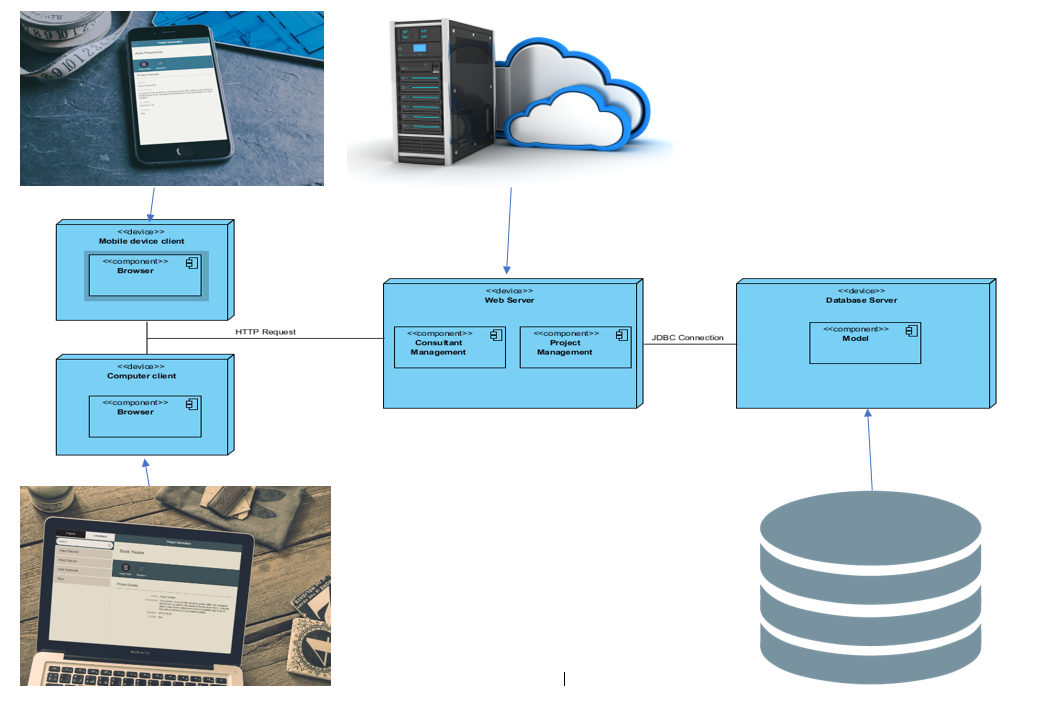
\includegraphics[width=\linewidth]{images/deploymentPic.PNG}

  \caption{Deployment Picture}

  \label{fig:sfig1}

\end{figure}

\section{Installation}

Upon project completion, no installation will be required to run the application as it will be available online.
Currently, one needs to download the source code from the Code Dynamic master branch on Github. The downloaded files can then be imported to Eclipse and run hosted locally on a Tomcat server.


\section{Getting Started}

The current implementation is based on the functional requirements of an administrator. The login/logout system has not been implemented yet, thus there are no section access restrictions.


\section{Using the system}

\subsection{Create Project}

The Administrator (Admin) clicks on the “Add” button on the bottom left corner of the User Interface (UI). A form appears where they have to fill in project details. The admin clicks the “Submit” button to save the project.

\begin{figure}[h]

\centering

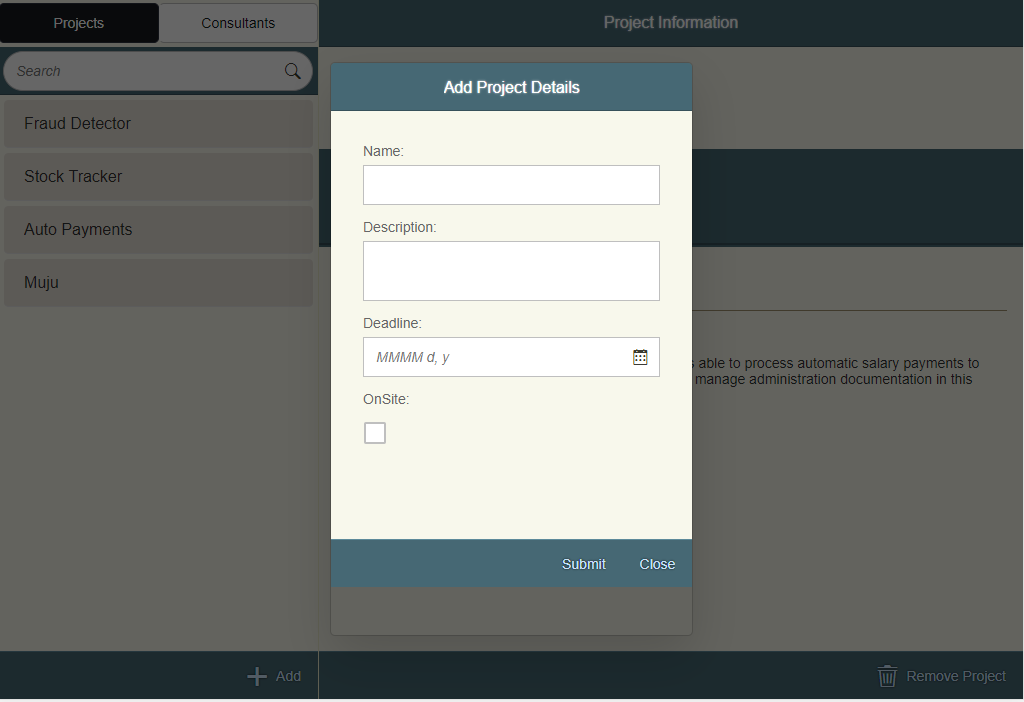
\includegraphics[width=\linewidth]{images/createProject.PNG}

\caption{Creating Project}

\label{fig:sfig1}

\end{figure}


\subsection{Delete Project}

The admin clicks on the “Remove Project” button on the  bottom right corner of the UI. A dialogue appears asking them to confirm their action. Clicking the “Delete” button deletes the project.

\begin{figure}[h]

\centering

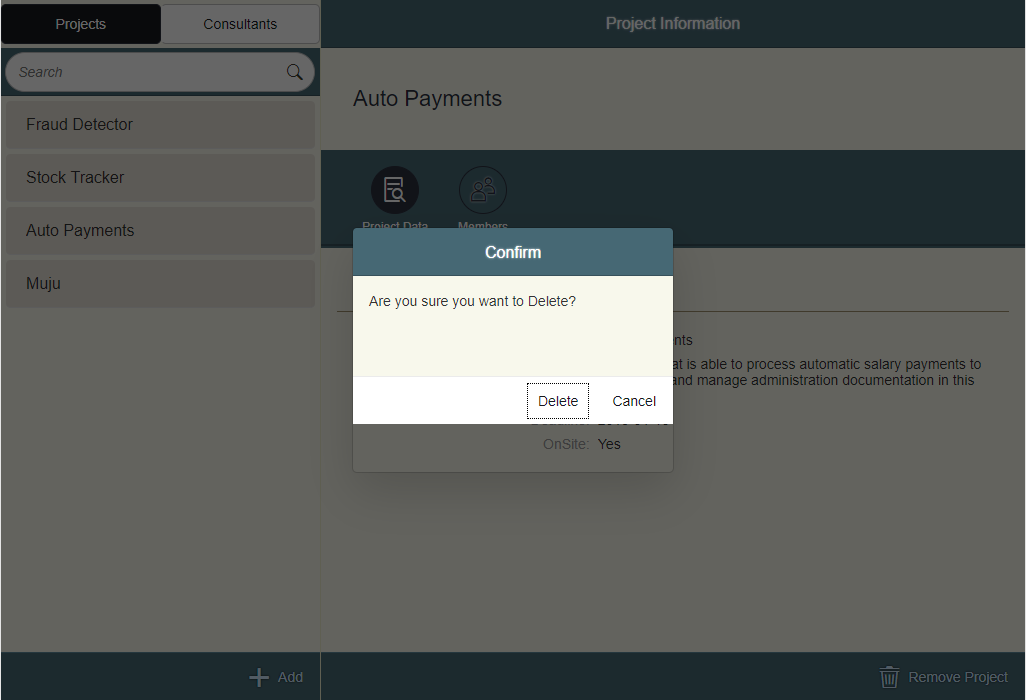
\includegraphics[width=\linewidth]{images/deleteProject.PNG}

\caption{Delete Project}

\label{fig:sfig1}

\end{figure}


\subsection{Create Consultant}

The admin clicks on the “Add” button on the bottom left corner of the UI. A form appears where they have to fill in product details. The admin clicks the “Submit” button to save the project.

\begin{figure}[h]

  \centering

  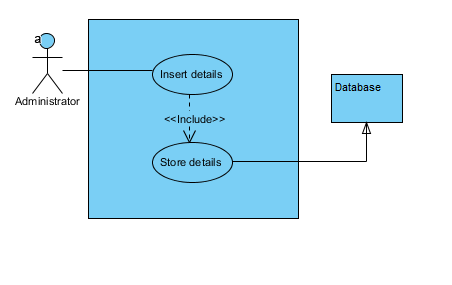
\includegraphics[width=\linewidth]{images/createConsultant.PNG}

  \caption{Create Consultant}

  \label{fig:sfig1}

\end{figure}


The admin clicks on the “Add Consultant” button on the right end of the UI. A dropdown with all the available consultants is shown. The admin selects 1 consultants and clicks the "Add" button.

\begin{figure}[h]

  \centering

  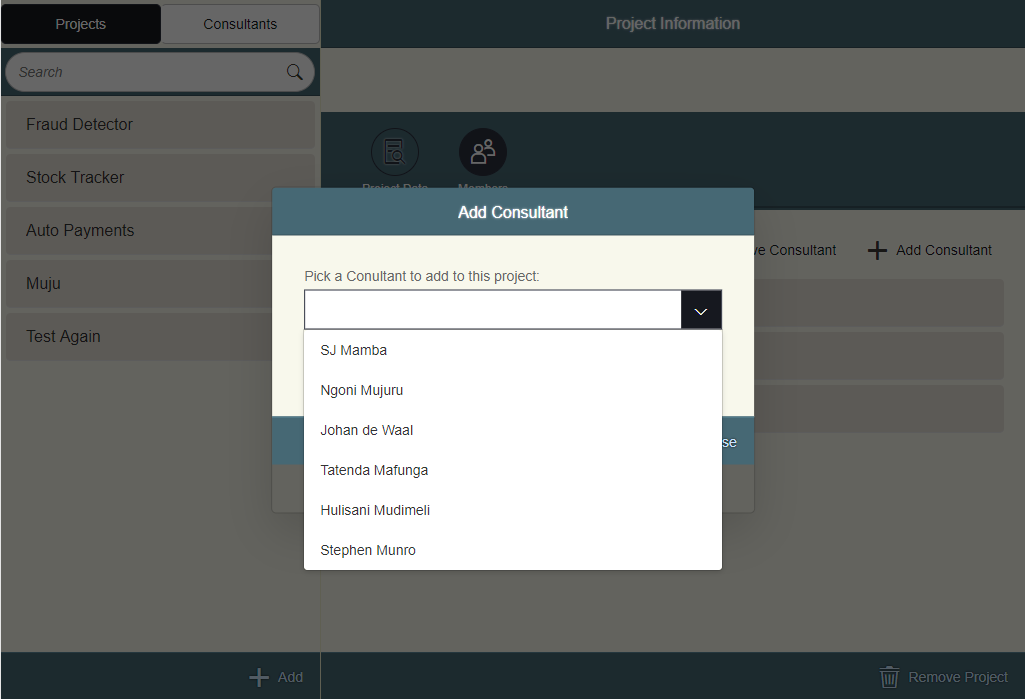
\includegraphics[width=\linewidth]{images/addConsultant.PNG}

  \caption{Add Consultant to Project}

  \label{fig:sfig1}

\end{figure}

\subsection{View Project}

The admin clicks on the “Projects” button on the top left section of the UI. A list of projects appears beneath the button. Clicking on any of the projects listed reveals the project information.

\begin{figure}[h]

  \centering

  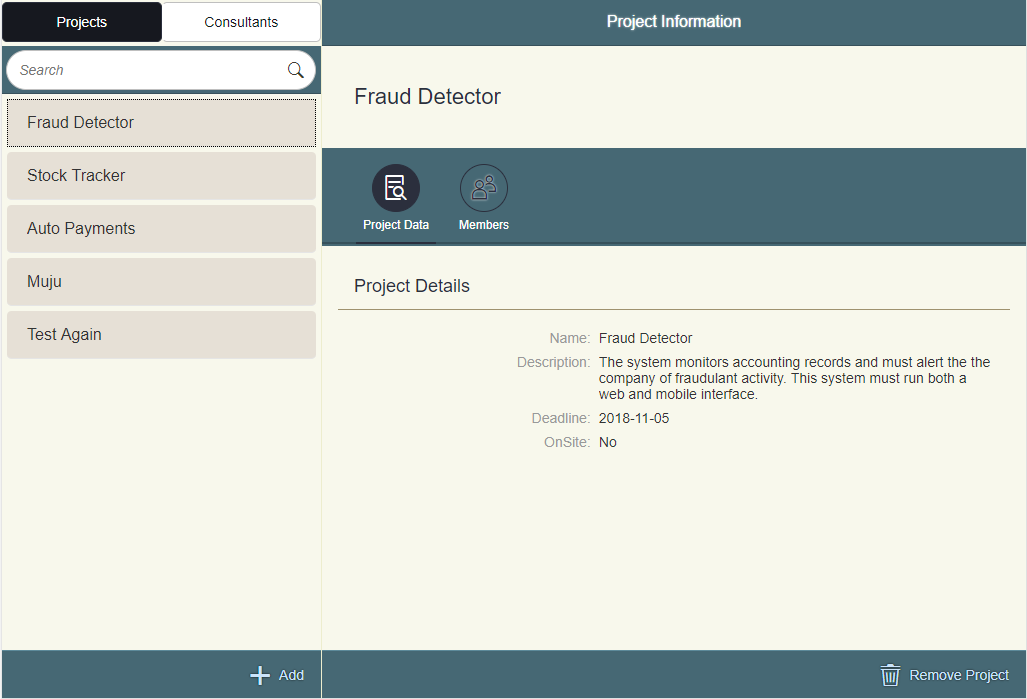
\includegraphics[width=\linewidth]{images/viewProject.PNG}

  \caption{View Project}

  \label{fig:sfig1}

\end{figure}

\subsection{View Consultant}

The admin clicks on the “Consultants” button on the top left section of the UI. A list of projects appears beneath the button. Clicking on any of the consultants listed reveals the selected consultants information.

\begin{figure}[h]

  \centering

  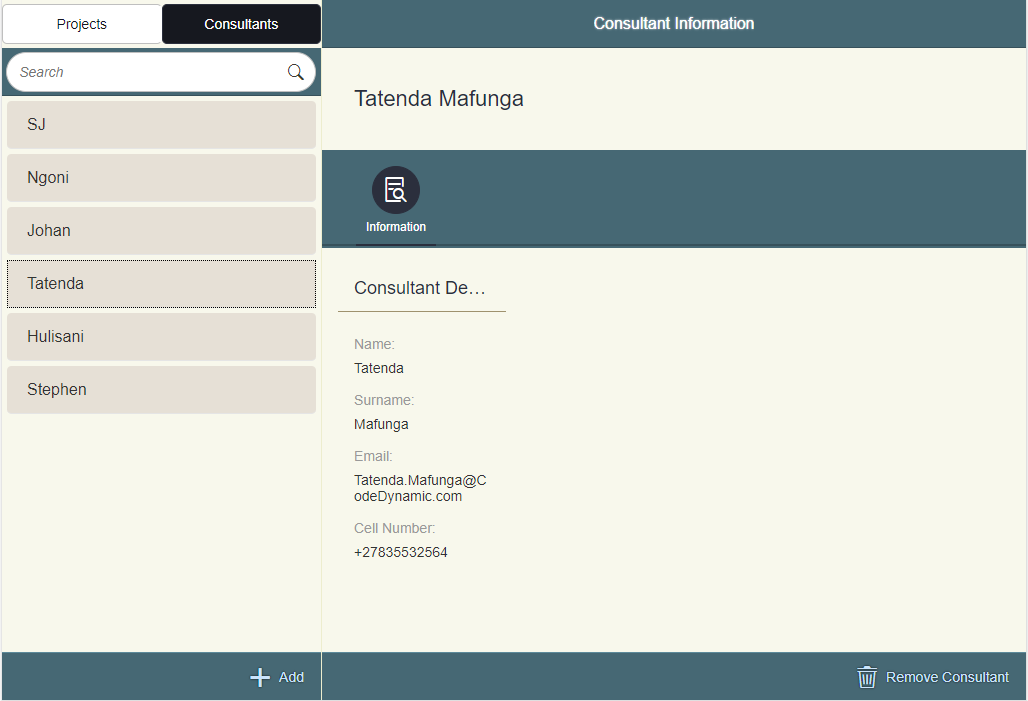
\includegraphics[width=\linewidth]{images/viewConsultant.PNG}

  \caption{View Consultant}

  \label{fig:sfig1}

\end{figure}



\section{Troubleshooting}

To be implemented at a later stage.

\end{document}
